\documentclass[]{article}
\usepackage[utf8]{inputenc}
\usepackage{graphicx}
\usepackage{amsmath}
\usepackage{amsfonts}
\usepackage{amssymb}
\usepackage{subcaption}
%opening
\title{Homework 4}
\author{Ian Hunt-Isaak}
\date{}
\begin{document}

\maketitle


\section{Introduction}
One of the fundamental problems of Quantum Mechanics is to calculate the eigenenergies of a given potential. On approach to calculating these values is to use the Imaginary time Schrödinger Equation (ITSCE). When the Schrödinger Equation is transformed to the imaginary time domain it can be rearranged into the familiar form of the Diffusion Reaction equation, which allows the propogation in time of the equation 
\section{Theory}
\subsection{Imaginary Time SCE}
With $H = T + V(x)$ the time independent SCE is:
\begin{equation}
H \phi_i(x) = \epsilon_i\phi_i(x)\text{, }i=0,1\dots
\end{equation}
where the $\epsilon_i$ are the eigen-energies, and $\phi_i$ are the eigenfunctions. 

One approach to find the eigen energies is begin with the time dependent SCE:
\begin{equation}
i\frac{\partial\psi(x,t)}{\partial t} = H\psi(x,t),
\end{equation}
and to use the transformation $\tau = i t$ resulting in the equation:

\begin{equation}
-\frac{\partial\psi(x,\tau)}{\partial t} = H\psi(x,\tau),
\label{eq:itsce}
\end{equation}
which has solution:
\begin{equation}
\psi(x,\tau) = e^{-\tau H}\psi(x,0).
\label{eq:this_one}
\end{equation}
If we decompose the initial wavefunction into a super position of eigen functions:
\begin{equation}
\psi(x,0) = \sum_{n=0}^{\inf}c_n \phi_n,
\end{equation}
then we can rewrite Eq. \ref{eq:this_one} as:
\begin{equation}
\psi(x,\tau) = \sum_{n=0}^{\inf}c_n e^{-\epsilon_n \tau}\phi_n.
\end{equation}
As $\epsilon_0 < \epsilon_n\text{, }n=1,2\dots$ we know that after a large time period the only eigenfunction significantly contributing to $\psi(x,\tau)$ will be that will with the lowest $\epsilon_n$. At this point the magnitude of the wave function will decrease as $e^{-\tau \epsilon_0}$, and we should not expect other oscillatory effects as we will have relaxed into the ground state, which is an eigenstate. Thus, if we can numerically propagate Eq. \ref{eq:this_one} in time and track the magnitude of a simulation point we can fit the decay of the magnitude at that point to extract the energy of the ground state.



In order to propagate Eq. \ref{eq:this_one} easily we can note that when substituting $H=T + V$ into Eq. \ref{eq:itsce} we get an equation of the same form as the Diffusion-Reaction equation. This is a form for which numerical solutions have been well explored, with many possible options such as forward Euler time stepping or the Lax-Wendroff method.

Of course it is often not just the ground state that is of interest. In order to compute the excited states we follow the same procedure as for the ground state but with an initial wavefunction that is orthogonal to the ground state wavefunction. We can construct such a wavefunction by taking our initial wavefunction used to find the ground state, $\psi^*(x)$, and subtract $c_0 \phi_0$. This is possible because at the end of the simulation used to find the ground state energy the wavefunction will be composed entirely of an un normalized $\phi_0$. We can find $c_0$ by taking:
\begin{equation}
\langle \psi^* | \phi_0 \rangle = c_0,
\end{equation}  
so we construct a new initial wavefunction as 
\begin{equation}
	\psi(x,0) = \psi^* - c_0*\phi_0,
\end{equation} 
and repeat the process. This is duplicable for all the excited states.
\subsection{Simple Harmonic Oscillator}
The simple harmonic oscillator has potential:
\begin{equation}
V(x) = \frac{1}{2}kx^2,
\label{eq:sho-v}
\end{equation}
for which the eignenergies have the well known form:
\begin{equation}
\epsilon_n = (n+\frac{1}{2})\hbar\omega.
\end{equation}
However, when working in natural units as in the simulations for this work the salient point to be taken from the energy formula is the ratio of successive energy states. Namely:
\begin{equation}
\epsilon_i = \epsilon_{i-1}, \text{ }i=1,2,\dots
\end{equation}
with $\epsilon_0 = 1$
\subsection{Infinite Square Well}
For the infinite square well potential:

\begin{equation}\label{ch:five:sec:5:eq4:1}
V(x)=
\begin{cases} 
0 & |x| < L/2 \\
\inf & \text{otherwise}
\end{cases}
\end{equation}
where L is the size of the well. The eigen-energies will scale as $n^2$:
\begin{equation}
\epsilon_n = \frac{n^2\pi^2\hbar^2}{2mL^2}.
\end{equation}
\section{Simulation Results}
\subsection{Simple Harmonic Oscillator}
For the SHO potential I started with the following wavefunction:
\begin{equation}
(1+r_1 x+r_2 x^2+r_3 x^3+r_4 x^4)e^{-x^2},
\end{equation}
where each $r_i$ is a random number between 0 and 1. A typical initial wavefunction can be seen in figure \ref{fig:sho_gs_init}. This form was used so that the wavefunction would go to zero as $x\to \pm\inf$ and to ensure that this guess was was composed of a superposition of the first several eigenfunctions. As expected the wavefunction decays towards the ground state wavefunction as seen in figure \ref{fig:gs_sho_decay}. By waiting until the wavefunction was centered  and then tracking the exponential decay of the points I found $\epsilon_0=1$ in the units I am working in, which makes sense. I then took the final time step from this simulation to be an unnormalized $\phi_0$ and used this to calculate the initial wavefunction to use in calculating the first excited state. This can be seen in figure \ref{fig:sho_excited_init}, I then propagated this as in Figure \ref{fig:sho_excited_decay}. Not only did the wavefunction have the correct qualitative shape but the energy $\epsilon_1$ was calculated as 3, which is consistent with the expected analytic ratio of $\frac{\epsilon_1}{\epsilon_0}$

\begin{figure}
	\centering
	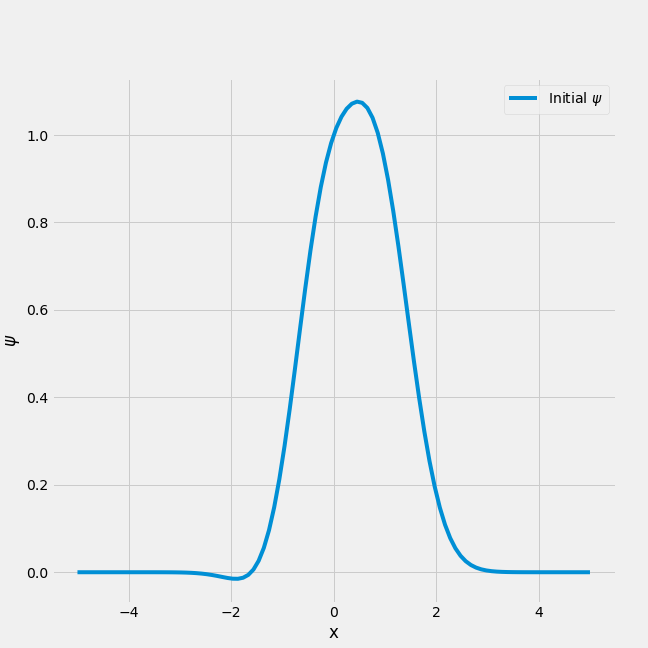
\includegraphics[width=.8\textwidth]{figures/ground_state_init.png}
	\caption{Typical initial wavefunction used to calculate the ground state of the SHO.}
	\label{fig:sho_gs_init}
\end{figure}
\begin{figure}
	\centering
	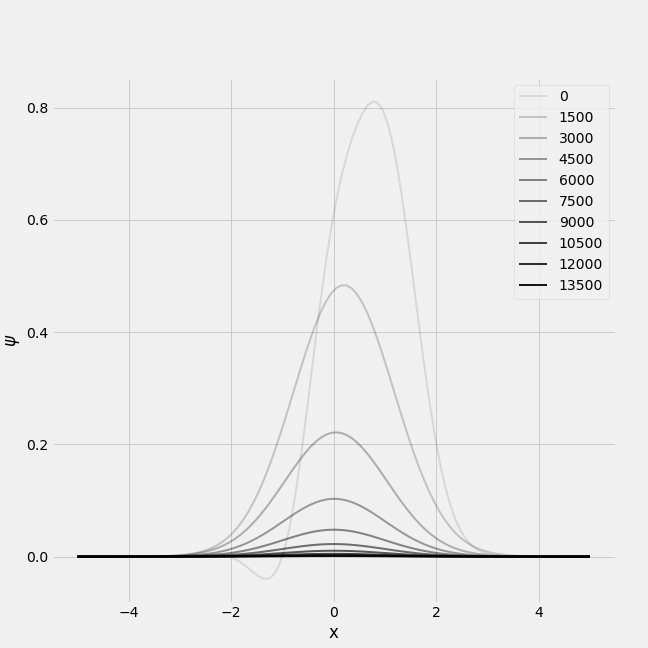
\includegraphics[width=.8\textwidth]{figures/ground_state_decay.png}
	\caption{The decay of the wavefunction with increasing $\tau$ when calculating the ground state of the SHO.}
	\label{fig:sho_gs_decay}
\end{figure}
\begin{figure}
	\centering
	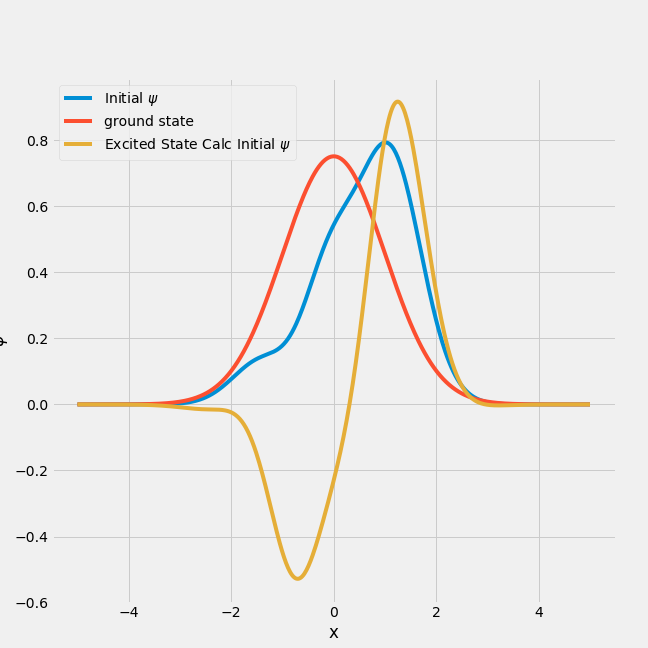
\includegraphics[width=.8\textwidth]{figures/excited_init.png}
	\caption{Calculation of the initial wavefunction to use for the calculation of the first excited state of the SHO. Each wavefunction plotted here has been normalized which is why the initial wavefunction for the first excited state has an extreme above the intial $\psi$.}
	\label{fig:sho_excited_init}
\end{figure}
\begin{figure}
	\centering
	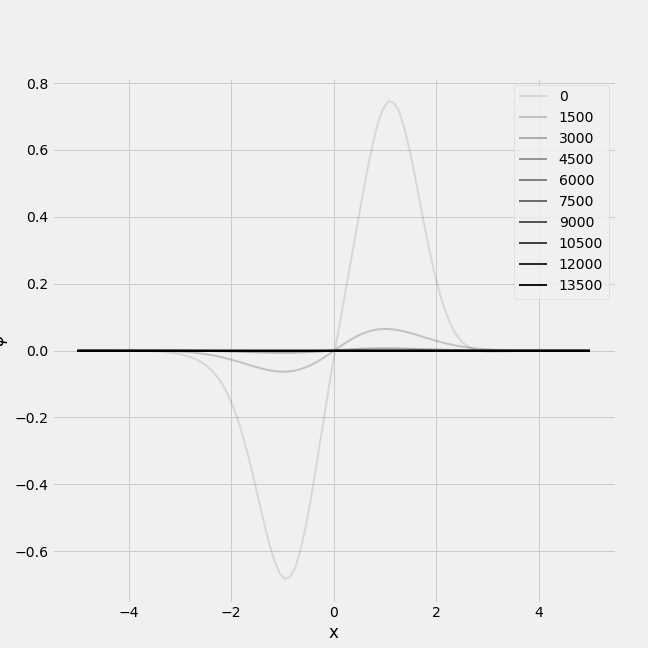
\includegraphics[width=.8\textwidth]{figures/e1_state_decay.png}
	\caption{The decay of the wavefunction with increasing $\tau$ when calculating the first excited state of the SHO.}
	\label{fig:sho_excited_decay}
\end{figure}


Unfortunately when I went to calculate the 2nd excited state I was unable to extract an energy other than the first excited state. I believe that this is a consequence of not have fully reached $\phi_1$ during my calculation of the first excited state. Indeed the wavefunction I took as as $\phi_1$ can be seen in figure \ref{fig:phi1} to clearly not be approriately symmetric. I took this as close enough as it gave me an energy of 3.03 which seemed to good enough, however clearly I should have run the simulation for many more iterations until assuming that I had reached $\phi_1$. An issue with this is the decay of the function to very small values, a possible workaround this problem would be renormalize the wavefunction at some point in the simulation and then continue to chart the decay. 
\begin{figure}
	\centering
	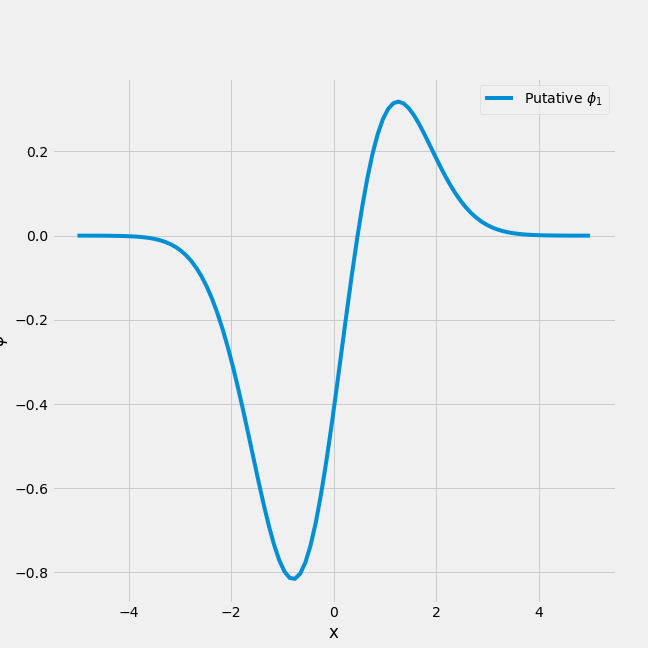
\includegraphics[width=.8\textwidth]{figures/phi1.png}
	\caption{The wavefunction that I used as $\phi_1$ when attempting to calculate the 2nd excited state. This clearly has not fully reached the eigenstate as can be seen from the assymetry about the y axis.}
	\label{fig:phi1}
\end{figure}


I found similar results with the Infinite square well.
\end{document}
